\chapter{Estabilidad del sistema de Lotka-Volterra generalizado}

\setlength{\parindent}{0cm} El capítulo anterior motiva al actual para presentar los resultados de la dinámica que produce el sistema de Lotka-Volterra generalizado (\ref{eqn:LK}) bajo los coeficientes de interacción de la matriz de incidencias (\ref{eqn:MatrizIncidencias}) para posteriormente linearizarlo mediante la Matriz Jacobiana del sistema (\ref{eqn:MartizJacobiana}). En este capítulo se presentarán los resultados que produce cada etapa del proceso, así como sus características. El objetivo será dar respuesta a cada una de las hipótesis del planteamiento del problema, sobre todo indagar las condiciones de estabilidad del sistema en términos de $\Lambda$ y reforzar la idea consecuente de la proposición \ref{prop:paramMay} en la que se detallaba que el parámetro de May (\ref{eqn:paramMay}) no necesariamente se ajusta a la estabilidad del sistema de Lotka-Volterra.\\
\\
Se consideraron 3 conjuntos diferentes de simulaciones: sistemas para 25, 50 y 100 especies. Para explorar los resultados se dejaron fijos la mayor cantidad de parámetros que hay en (\ref{eqn:LK}) con el fin de observar cambios significativos con la menor cantidad de fluctuaciones posibles; únicamente se han variado las matrices de incidencias $\Lambda$ que dependen de $p$ y $\sigma$, y al igual que en las transiciones de May se varió una de estas cantidades mientras que la otra permaneció fija. En todas las simulaciones la tasa de crecimiento se dejó fija en $r=2$ y la capacidad de carga en $K=5$ para toda especie del sistema. Al integrar numéricamente las ecuaciones con RK4 se escogió un intervalo de tiempo entre 0 y 50 con un paso de integración de $h=0.01$.\\
\\
Además de estos parámetros, siempre se inicializó cada simulación con la condición inicial $\vec{x}_0=\vec{1}$ (según el tamaño del sistema) y se consideraron dos escenarios\footnote{solo aplicca para $N=100$, el resto de casos se consideraron $\Lambda$ estructuralmente simétricas.}: Matrices de incidencias estructuralmente simétricas y puramente aleatorias, tal y como se visualizó al final del capítulo anterior. En el apéndice (\ref{ch:Ap}), el lector puede darse una idea de como se realizó el proceso de las simulaciones. En cada escenario se presentó cierta cantidad de ruido en las gráficas de estabilidad, por lo que el número de simulaciones fue establecido en función de la disminución de dicho ruido (haciendo uso de la ley de los grandes números).

\section{Series de tiempo}

Anteriormente se ha comentado que las interacciones de la matriz de incidencias $\Lambda$ están volteadas con respecto de la matriz de Jacobiana del sistema $\mathcal{J}$; por ejemplo, la cooperación en $\mathcal{J}$ se da para las interacciones (++) mientras que para $\Lambda$ es $(--)$. La propia definición de la Jacobiana garantiza este hecho. Si se tuviera un sistema puramente de competencia, es decir para toda $\alpha_{ij}\in\Lambda$ mayor o igual que cero, entonces no hay forma de que ninguna de las poblaciones participantes sobrepasen la capacidad de carga establecida, tal y como se indica en la ecuación (\ref{eqn:LKextendida}) y en el Ejemplo \ref{eg:2x2}. Por lo tanto obtendríamos series de tiempo caóticas para cada una de las especies por debajo de $K=5$.
\begin{figure}[h!]
	\centering
	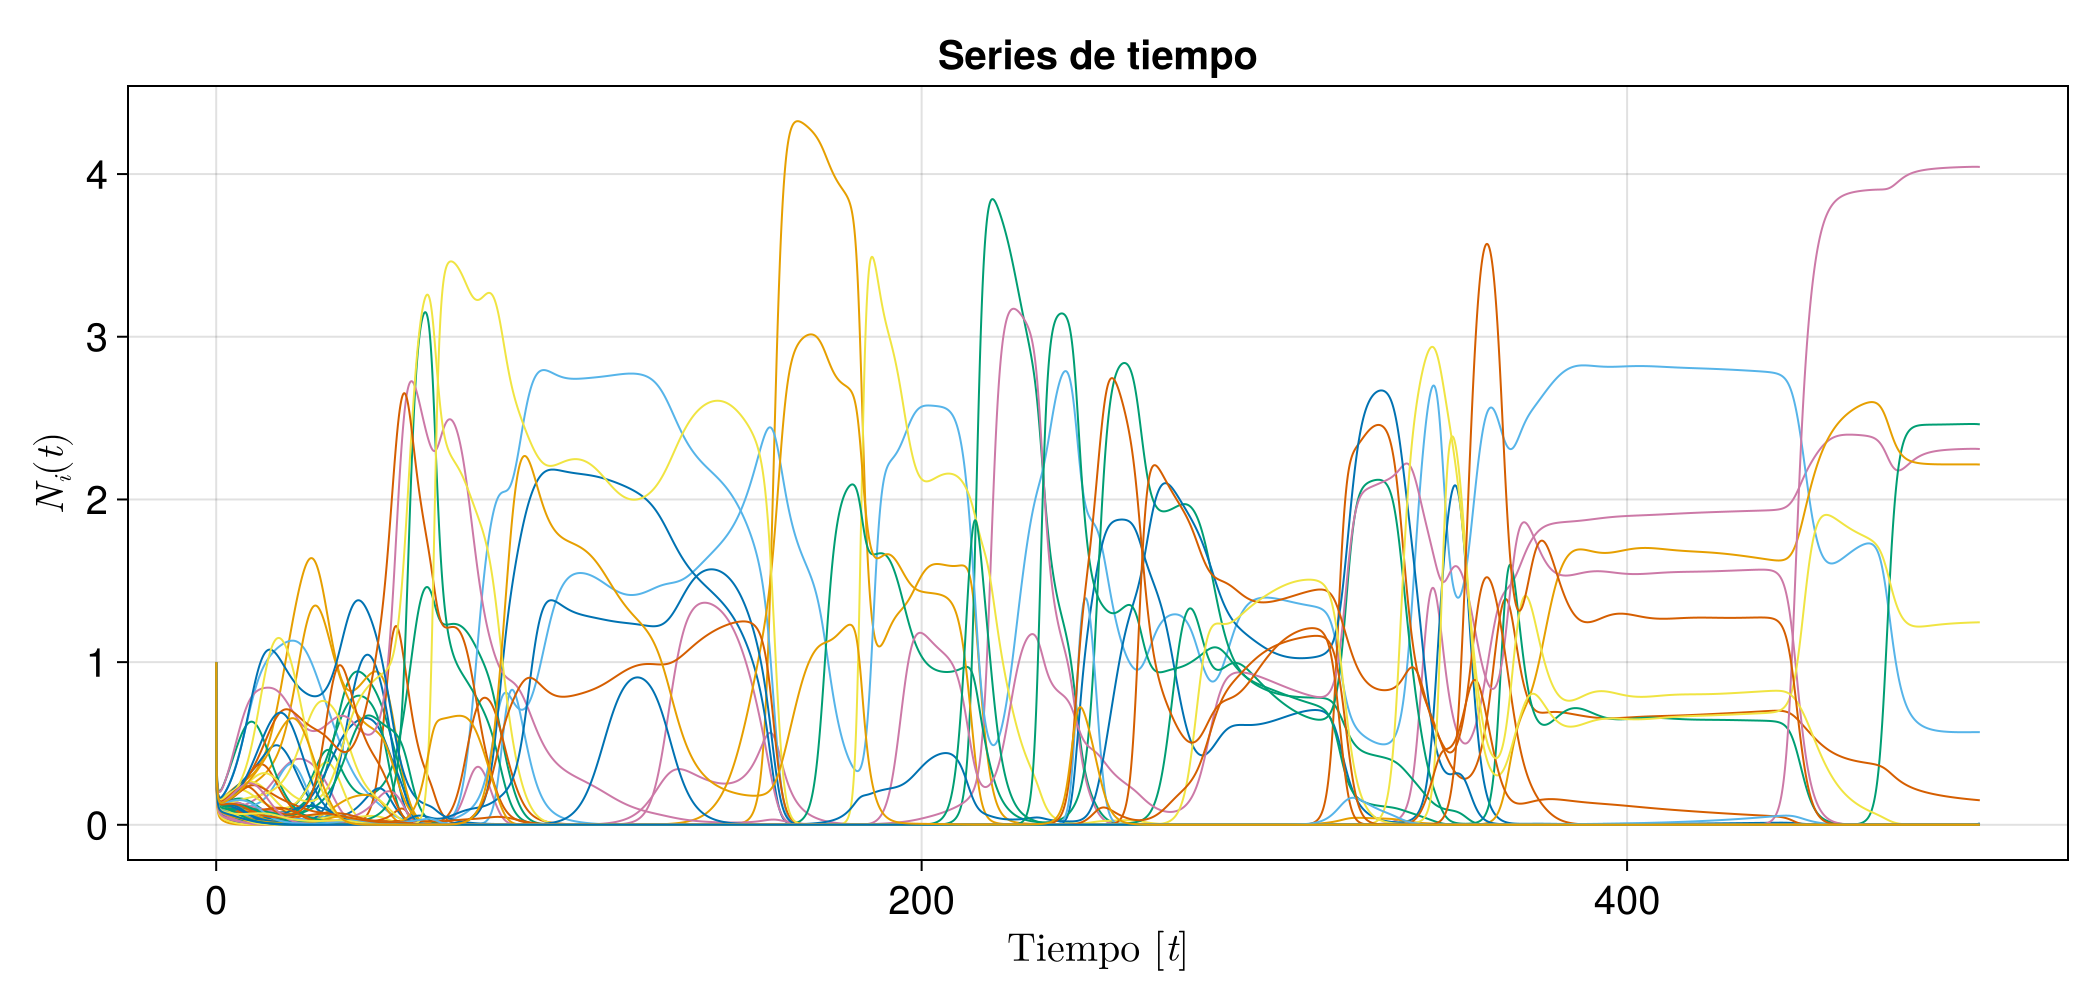
\includegraphics[scale=0.23]{../Imagenes/Seriesdetiempopositiva}
	\caption{Series de tiempo para el sistema de competencia de especies. Se emplea una matriz de incidencias para $N=100$ cuyas entradas vienen de una distribución uniforme del intervalo $[0,1]$. Se considera a la red completa con $p=1.0$, es decir, con el número máximo de enlaces posibles. En este caso la dinámica no sobrepasa la capacidad de carga puesto que las 100 especies se encuentran compitiendo y obedeciendo el comportamiento logístico que se muestra en (\ref{eqn:LKextendida}).}
	\label{fig:Seriesdetiempopostiva}
\end{figure}

Una de las características que se encontró en esta clase de sistema en particular es que el tiempo en que tarda en estabilizarse es considerablemente mayor que en los sistemas donde se considerarán todas las interacciones antes mencionadas. Las poblaciones al estar confinadas por la capacidad de carga, tienen más oportunidad de interactuar entre sí, generando constantes fluctuaciones que prolongan el tiempo de estabilización.\\
\\
Por el contrario, el sistema generalizado sí excede la capacidad de carga lo que se traduce en una disminución de la cantidad de fluctuaciones debido a las especies dominantes que regulan el sistema y hace que lleguen al atractor en un tiempo menor. Otro aspecto que se encontró en la red de competencias es que cuando es más conectada tarda más tiempo en estabilizarse. Si se generara una red de competencias con pocas conexiones ($p\leq 0.5$) el número de especies que compiten es considerablemente menor, lo que implica que exista menor cantidad de fluctuaciones y por ende mayor facilidad para llegar a la estabilidad.\\
\\
En el Ejemplo \ref{eg:2x2CoopyDemás} del capítulo anterior, se observaba como las interacciones de cooperación $(--)$ en la matriz de incidencias $\Lambda$ genera la aparición de un atractor para ambas especies que se posiciona por arriba de la capacidad de carga (Figura (\ref{fig:CooperacionEspecies})). En el caso extendido a $N\gg 1$ especies ocurrirá algo semejante considerando un atractor $N$-dimensional. En este caso pueden haber especies que sobrepasen por mucho o poco la capacidad de carga, pero también cabe la posibilidad de que algunas no logren sobrepasarla y otras que lleguen a extinguirse. A continuación se muestran dos ejemplos diferentes
\begin{figure}[h!]
	\centering
	\includegraphics[scale=0.23]{../Imagenes/Series de Tiempo LK100}
	\caption{(\textbf{A}) Series de tiempo del sistema de Lotka-Volterra generalizado asociada a una matriz de incidencias de $N=100$, con $\sigma=0.2$ y $p=0.35$. (\textbf{B}) Series de tiempo para el sistema de Lotka-Volterra generalizado asociada a una matriz de incidencias de $N=100$ nodos con $\sigma=0.2$ y $p=0.5$}
	\label{fig:SeriesdeTiempoLK100}
\end{figure}

La diferencia evidente entre estas gráficas es debido la matriz de incidencias, sus parámetros son $\sigma=0.2$ con $p=0.35$ y $p=0.5$ respectivamente. El segundo caso corresponde con una red más conectada que el primero y eso se traduce en la oportunidad de tener más interacciones con signo negativo que propicien un mayor crecimiento. El tiempo en que llegaron a estabilizarse fue menor a $t=50$, y a su vez considerablemente menor que el sistema de competencia de especies de la Figura (\ref{fig:Seriesdetiempopostiva}). 
\\
\\
En un principio, los resultados de la Figura (\ref{fig:SeriesdeTiempoLK100}) se generaron sin tener un mapa de estabilidad únicamente teniendo como referencia el parámetro de May (\ref{eqn:paramMay}). Además de construir los mapas de estabildiad (que es lo que se hará más adelante), es de interés buscar un parámetro crítico de transición como el de May. Para ello será crucial conocer más sobre $\Lambda$, pues es quien realmente determina la estabilidad de los sistemas.

\subsection{Puntos fijos}

Como bien ya se sabe, los puntos fijos son aquellos en los que se refleja la estabilidad del sistema además de que son vitales para determinar la matriz Jacobiana del sistema de Lotka-Volterra generalizado. Sin embargo, serán los propios coeficientes de la matriz de incidencias los que definan si el sistema es estable o no. Esta conjetura podrá no ser trivial de abordar pero si es posible realizar un análisis exploratorio. Los puntos fijos del sistema se determinan de igualar a cero y resolver las ecuaciones (\ref{eqn:LK}) lo que sería equivalente tener el siguiente sistema
\begin{equation}\label{eqn:PuntoFijo}
	x_i=K_i-\sum_{j\neq i}\alpha_{ij}x_j
\end{equation}
considerando que $\alpha_{ii}=1$. Las soluciones que puede tener este sistema son múltiples, se pueden generar combinaciones de casos para poder resolverlo: por ejemplo igualar a cero un subconjunto de ecuaciones de este sistema ($x_{k}=0$) y resolver para dicha/s condición/es. Las soluciones favorables son para cuando todo elemento $x_i\in X$ del punto fijo es mayor o igual que cero; el sistema no restringe soluciones $x_k\in X$ negativas, pero no serán de interés puesto que no hay sentido físico en interpretar poblaciones negativas\footnote{Además de que los experimentos han arrojado sistemas inestables cuando el punto fijo $X$ tiene entradas negativas.}. Por último, de las soluciones favorables es de interés saber que condiciones en $\Lambda$ hace que el punto fijo sea estable o inestable.\\
\\
Para un primer análisis exploratorio, se utilizará aproximación de campo medio para realizar una estimación general de las soluciones del sistema. Para ello se considerará que toda $x_i\in\Lambda$ cumple $x_i\approx\langle x\rangle$, asumiendo esta hipótesis y aplicándola en (\ref{eqn:PuntoFijo}) se tiene
\begin{equation}
	\begin{split}
		&\langle x\rangle+\sum_{j\neq i}\alpha_{ij}\langle x\rangle=K_i\\
		&\langle x\rangle=\frac{K_i}{1+pN\sigma^2},\qquad 
	\end{split}
\end{equation}
considerando que $\sum_{j\neq i}\Var(\alpha_{ij})\approx pN\sigma^2$. Este resultado indicaría como son las soluciones del punto fijo en gran o en menor medida, de aquí en adelante se tendría el camino directo para poder estimar el parámetro de transición que tanto se espera sino fuera por algunos aspectos a considerar: La suposición de campo medio excluye soluciones negativas, lo cual se sabe que existen pero para ningún valor de $p$, $N$ y $\sigma$ se generan tales escenarios; el segundo aspecto a considerar es que de acuerdo a los ejemplos de la Figura (\ref{fig:SeriesdeTiempoLK100}), el punto fijo no sigue una distribución de campo medio, sino más bien una tendencia de distribución de cola pesada con sesgo positivo. \\
\\
El lector podrá comprobarlo una vez que haya seguido todos los pasos del apéndice para integrar el sistema. Además podrá comprobar que dicha distribución irá variando en función de los parámetros de $\Lambda$ lo cual también se deja ver un poco en las series de tiempo mencionadas. Una alternativa para poder estimar una solución tal y como se hacía considerando aproximación de campo medio sería adecuar este proceso para la distribución de cola pesada. Suponer campo medio es considerar que las entradas del punto fijo siguen una distribución normal, la idea en este caso sería caracterizar estas distribuciones de cola pesada con alguna ya conocida y aplicar campo medio bajo la hipótesis de esta nueva distribución.\\
\\
Teniendo contexto de la distribución de las entradas del punto fijo (mediante las series de tiempo generadas) y de los coeficientes de $\Lambda$ que inducen a dicha distribución, se podrá acceder a la información necesaria para determinar que condiciones generan sistemas de Lotka-Votlerra generalizados estables. Pero por el momento el análisis quedará hasta aquí esperando que las ideas se retomen más adelante.

\section{Matriz Jacobiana}

Anteriormente se ha definido la matriz Jacobiana del sistema de Lotka-Volterra generalizado (\ref{eqn:MartizJacobiana}), para que surta efecto es necesario conocer el punto fijo de interés y se hará por medio de la serie de tiempo tal y como aparece en la Figura (\ref{fig:SeriesdeTiempoLK100}). Se recolecta la última entrada de la serie, asumiendo que es un punto fijo estable, y se guarda como vector $N$-dimensional para poderse evaluar en la matriz Jacobiana. Para validar el resultado solamente resta calcular sus valores propios y confirmar la estabilidad por medio de la parte real de los mismos. Por otro lado, si la serie de tiempo diverge entonces se asume que el sistema es inestable.
\\
\\
Un elemento importante de este proceso es que no es trivial determinar cuando se estabilizará el sistema por medio de la serie de tiempo, en general se ha observado que gran porcentaje de los sistemas se estabilizan en un tiempo menor o igual a $t=50$, sin embargo, existen sistemas que se estabilizan en un tiempo superior a este lo que ha generado algunos detalles en los resultados obtenidos. En este sentido, se han observado casos en los que se extrae el punto fijo que aparenta ser estable pero al determinar la estabilidad por medio de los valores propios de la matriz Jacobiana se encuentra que  algunos de ellos tienen parte real positiva lo que induce a sistemas inestables. Para evitar que esto ocurra es importante incluir una restricción sobre el tiempo de integración, recolectar sistemas que se estabilicen en un tiempo menor o igual a $t=50$.
\\
\\
Comenzando con el análisis de los resultados obtenidos, se han generado cuatro ejemplos arbitrarios para ir observando las características de las matrices Jacobianas de los sistemas (\ref{eqn:LK}) que resultaron estables. En este \href{https://github.com/rogve98/Tesis/tree/master/Notebooks/Datos/Ejemplo\%20Jacobianos}{enlace}\footnote{Consultar: \url{https://github.com/rogve98/Tesis/tree/master/Notebooks/Datos/Ejemplo\%20Jacobianos}} el lector tendrá acceso a 4 de estas matrices para los parámetros $N=100$, $\sigma=0.2$ y $p=\{0.3,0.4,0.5,0.6\}$. A continuación se presenta el código en \julia para validar si las diagonales de cada matriz Jacobiana son negativas siguiendo la Poposición \ref{prop:DiagonalI}
\begin{tcolorbox}[colback=green!10!white, colframe=black, title=Entrada]
	\begin{minted}{julia}
using CSV, DataFrames
jacobianos = []
for i in 0.3:0.1:0.6
    ruta = "Datos/Ejemplo Jacobianos/Jacobiano100_p$i.s0.2.csv"
    df = CSV.read(ruta,DataFrame,header=false)
    push!(jacobianos,df)
end
jacobianos
	\end{minted}
\end{tcolorbox}

\begin{tcolorbox}[colback=red!10!white, colframe=black, title=Salida]
4-element Vector{Any}:\\
100×100 DataFrame
\end{tcolorbox}

Validando las diagonales de cada uno de las matrices consideradas se tiene

\begin{tcolorbox}[colback=green!10!white, colframe=black, title=Entrada]
	\begin{minted}{julia}
using LinearAlgebra
print(all(x -> x<0,diag(Matrix(jacobianos[1]))),", ")
print(all(x -> x<0,diag(Matrix(jacobianos[2]))),", ")
print(all(x -> x<0,diag(Matrix(jacobianos[3]))),", ")
print(all(x -> x<0,diag(Matrix(jacobianos[4]))))
	\end{minted}
\end{tcolorbox}

\begin{tcolorbox}[colback=red!10!white, colframe=black, title=Salida]
true, true, true, true
\end{tcolorbox}
\newpage
El siguiente detalle a analizar siguiendo la definición de la matriz Jacobiana (\ref{eqn:MartizJacobiana}) es que sus diagonales en efecto no son homogéneas como en las matrices de May. Determinando un histograma de cada una de las diagonales de las matrices antes consideradas se puede saber como es su distribución y si cambia con respecto de la $p$ elegida
\begin{figure}[h!]
	\centering
	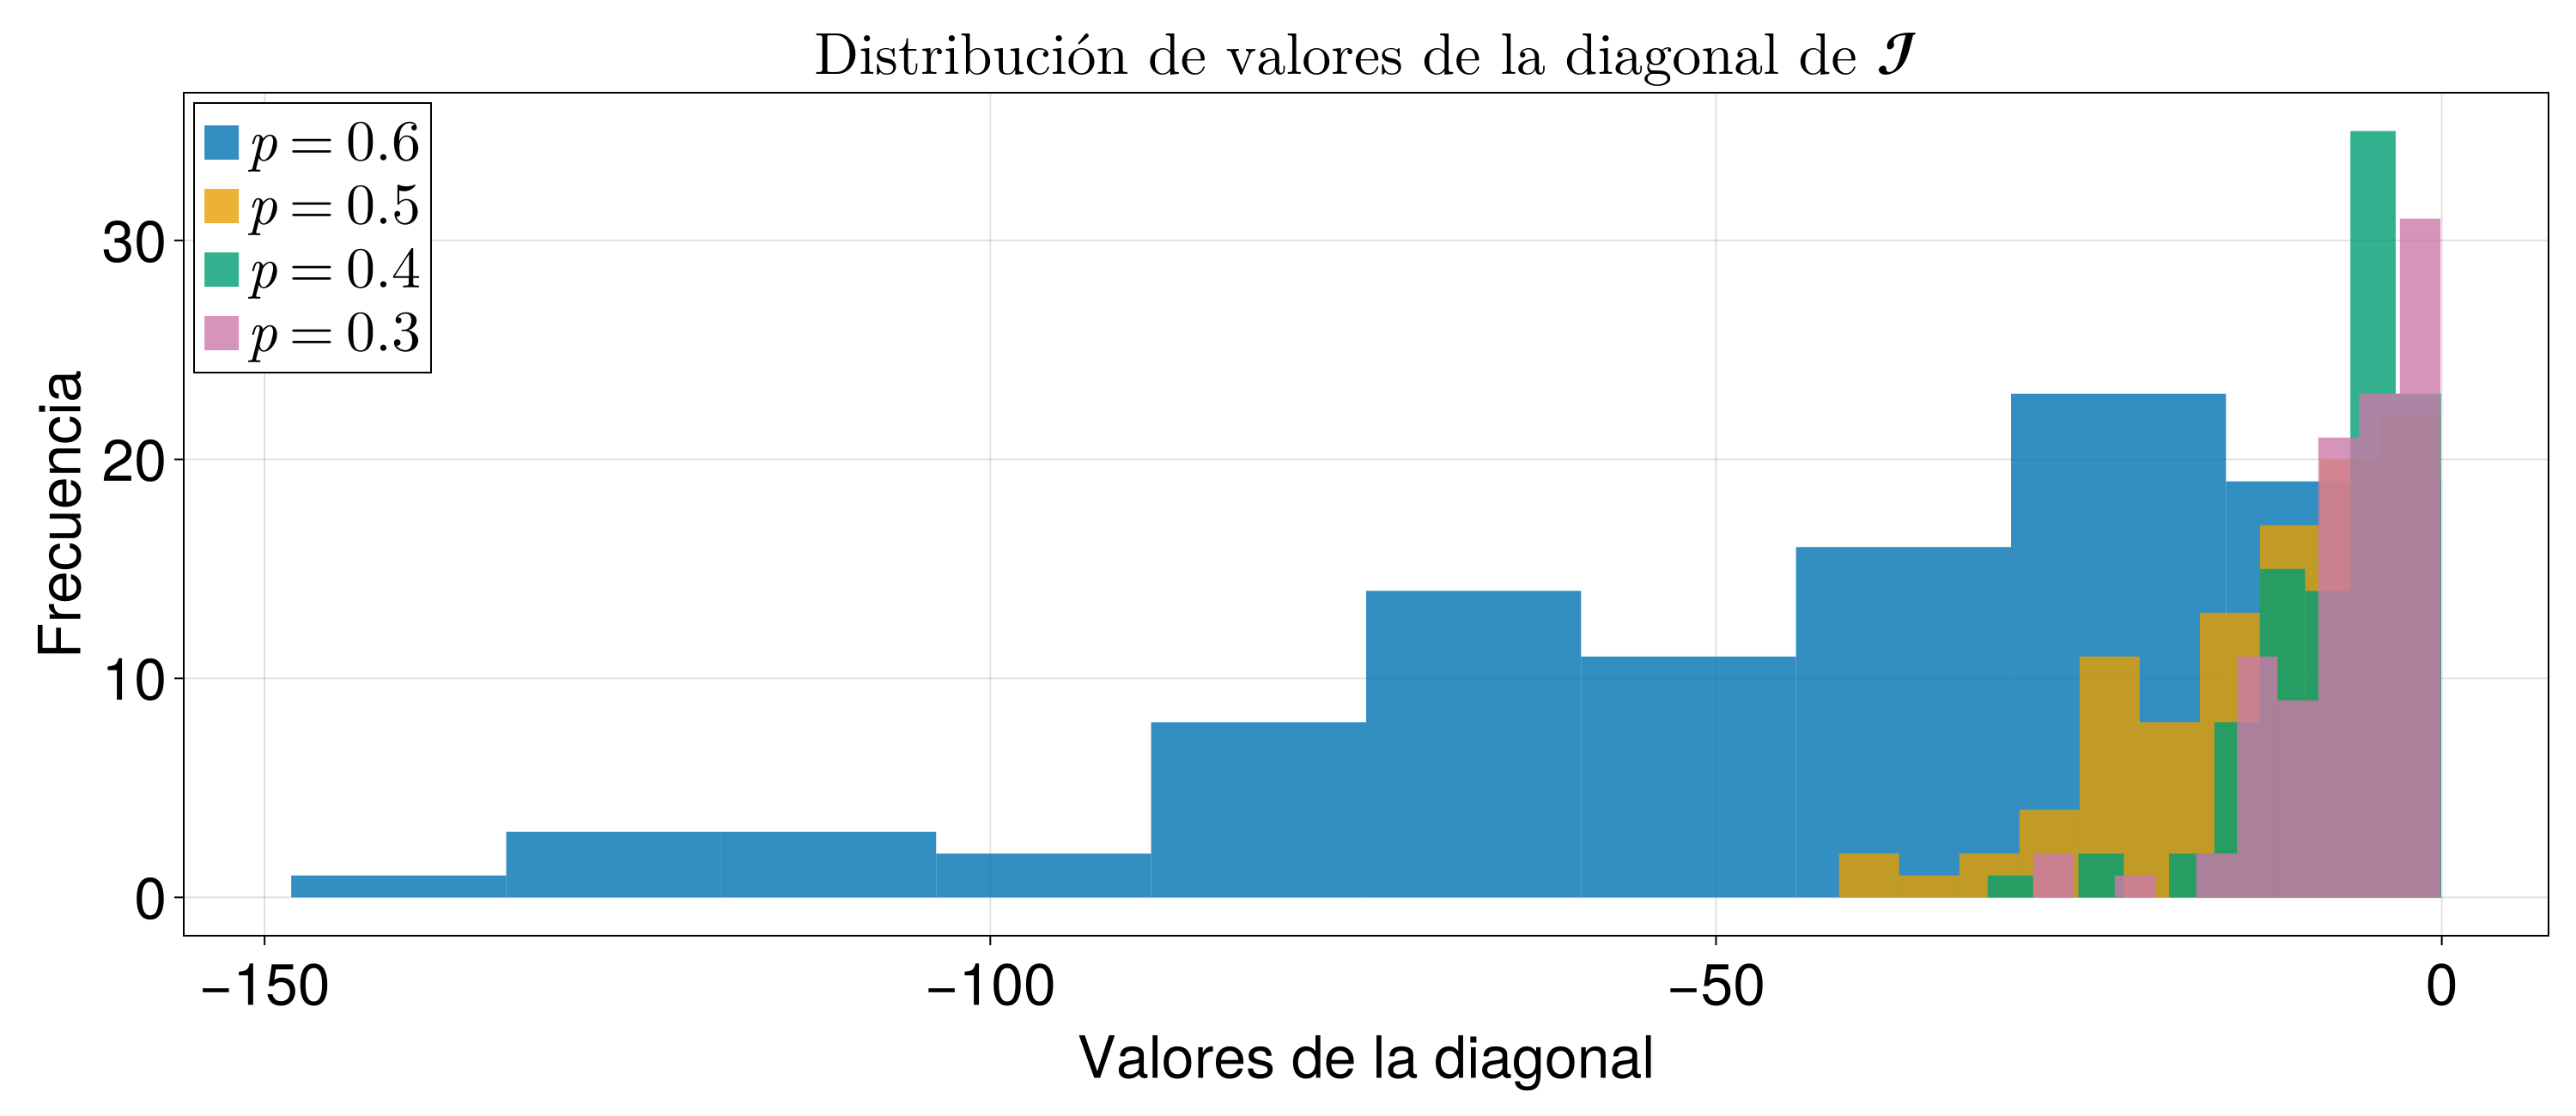
\includegraphics[scale=0.16]{../Imagenes/DistDiagonal}
	\caption{Distribuciones de diagonales de cada matriz Jacobiana antes considerada considerando para $N=100$, $\sigma=0.2$ y $p\in\{0.3,0.4,0.5,0.6\}$.}
	\label{fig:DistDiagonal}
\end{figure}

No solo no es homogénea sino que cuanto la probabilidad es mayor, la distribución es más dispersa hacia los valores negativos haciéndola de cola pesada tal como se observa el contraste entre el caso $p=0.6$ y $p=0.3$. Este comportamiento es natural considerando los coeficientes de $\Lambda$ y las entradas del punto fijo que también vienen de una distribución de cola pesada. Más adelante se discutirá acerca de esta cualidad de las distribuciones resultantes.
\\
\\
En el capítulo pasado se vio que la importancia de la diagonal en las matrices de May radica en la forma de la distribución de los valores propios del sistema en el plano complejo, englobado bajo la Ley Circular. En la Proposición \ref{prop:paramMay} se demostró que existen varios discos de Gershgorin centrados en este valor $-d$ de la diagonal, que encierran a los valores propios del sistema en el semiplano negativo de $\mathbb{C}$ y que el parámetro de May (\ref{eqn:paramMay}) determina el límite entre estabilidad e inestabilidad. En el caso de las matrices Jacobianas de los sistemas de Lotka-Volterra generalizado, al no tener un radio/centro definido debido a forma heterogénea de las diagonales ¿qué se puede esperar de la distribución de valores propios de $\mathcal{J}$?
\newpage

\section{Leyes Circulares}

Sabiendo que la distribución de la diagonal de las Jacobianas de los sistemas generalizados no es homogénea y que sigue una distribución de cola pesada con sesgo negativo, se debe analizar como es su distribución de valores propios en el plano complejo y si tiene alguna relación con la distribución de la diagonal. Para ello se comenzará por revisar la distribución de los valores propios de las matrices Jacobianas que se invocaron en la sección anterior
\begin{figure}[h!]
	\centering
	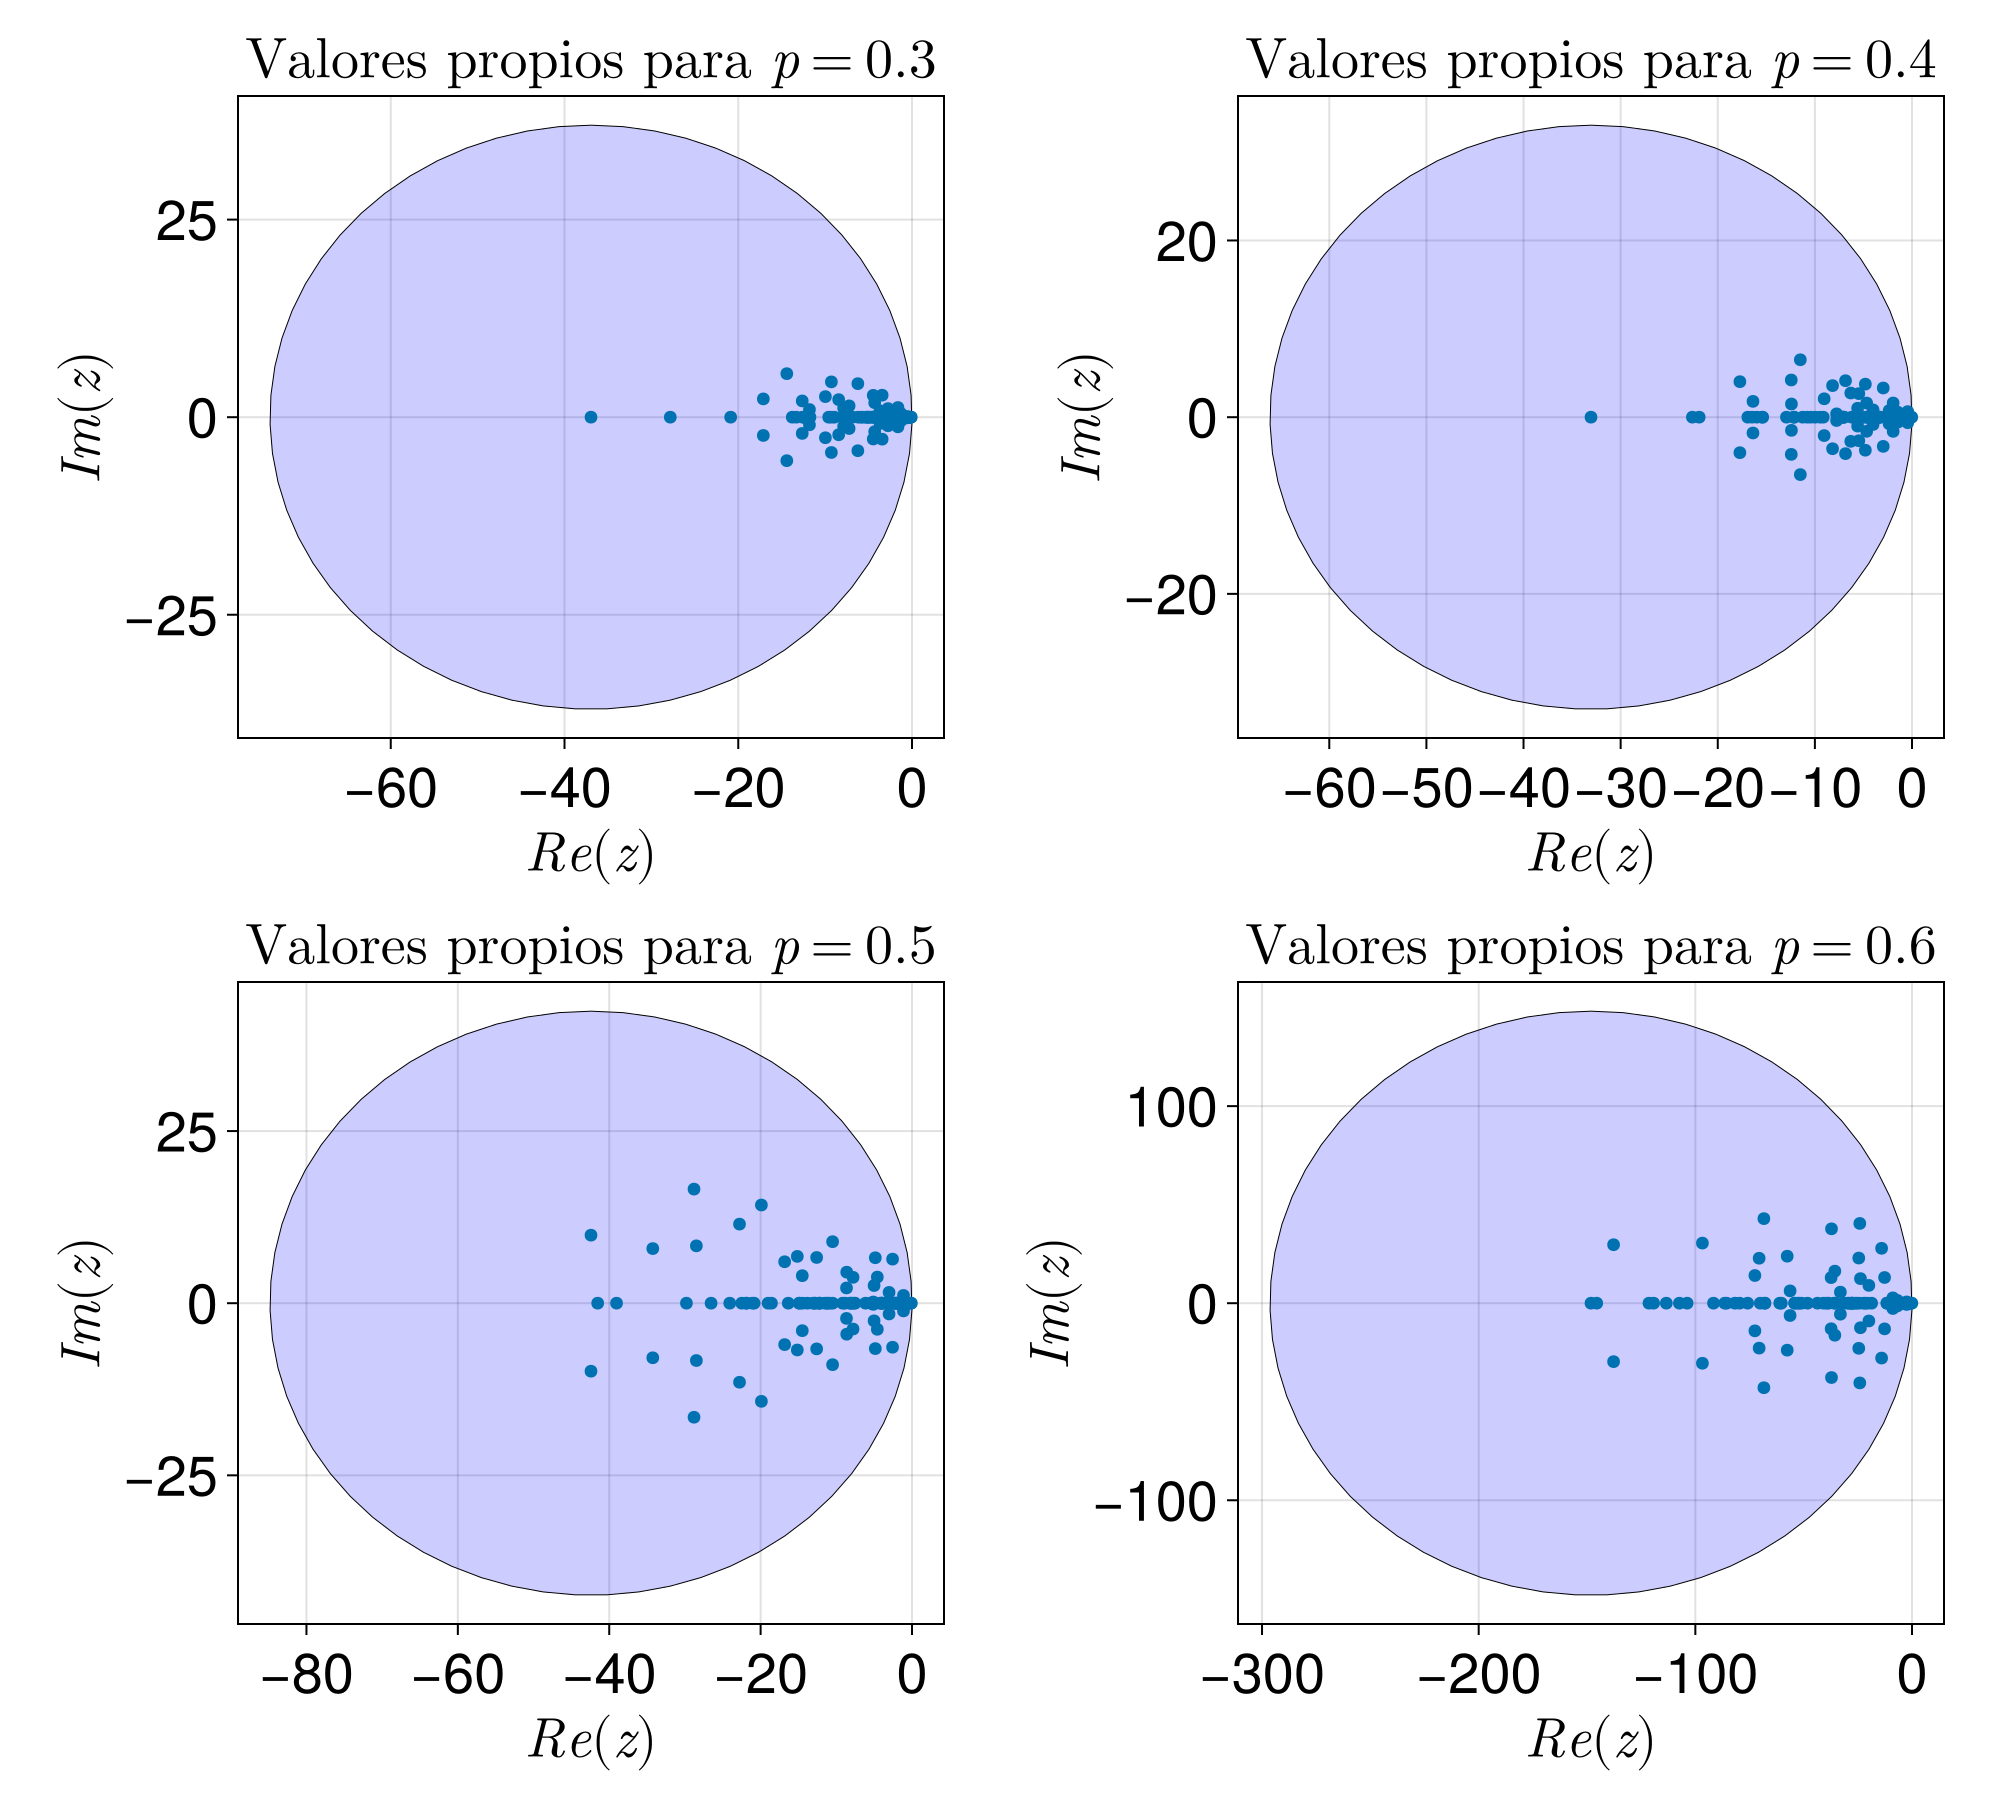
\includegraphics[scale=0.24]{../Imagenes/DistEigenvalores}
	\caption{Distribución de valores propios para el conjunto de Jacobianas antes consideradas con los parámetros $N=100$, $\sigma=0.2$ y $p\in\{0.3,0.4,0.5,0.6\}$.}
	\label{fig:DistEigenvalores}
\end{figure}

Para comenzar se han propuesto como centro y radio la parte real más negativa del conjunto de valores propios de cada ejemplo\footnote{En consecuencia se genera el Círculo con el radio más grande posible de cada sistema.}, y en primera instancia se puede observar que dichos círculos si encierran a cada una de las distribuciones pero no se ajustan al círculo en concreto. Además de que cada distribución se encuentra en el semiplano negativo de $\mathbb{C}$, se puede apreciar de cada distribución que cuando la probabilidad de conexión es mayor entonces  la distribución se ensancha desde el eje real de forma similar a como se observa en la Figura (\ref{fig:DistDiagonal}), lo que podría sugerir una relación entre la distribución de las diagonales de $\mathcal{J}$ y de sus valores propios. \\
\\
Es evidente que la distribución de la diagonal impacta directamente en la distribución de los valores propios, y si no hay una Ley Ciruclar que se ajuste a dicha distribución entonces se puede proponer la posibilidad de que existan $N$ de ellas. Para dar un acercamiento a esta propuesta, se ocupará la distribución más ancha para $p=0.6$ (de los ejemplos antes presentados) y se considerará cada valor de la diagonal de su matriz Jacobiana como centro y radio de una Ley Circular particular.
\begin{figure}[h!]
	\centering
	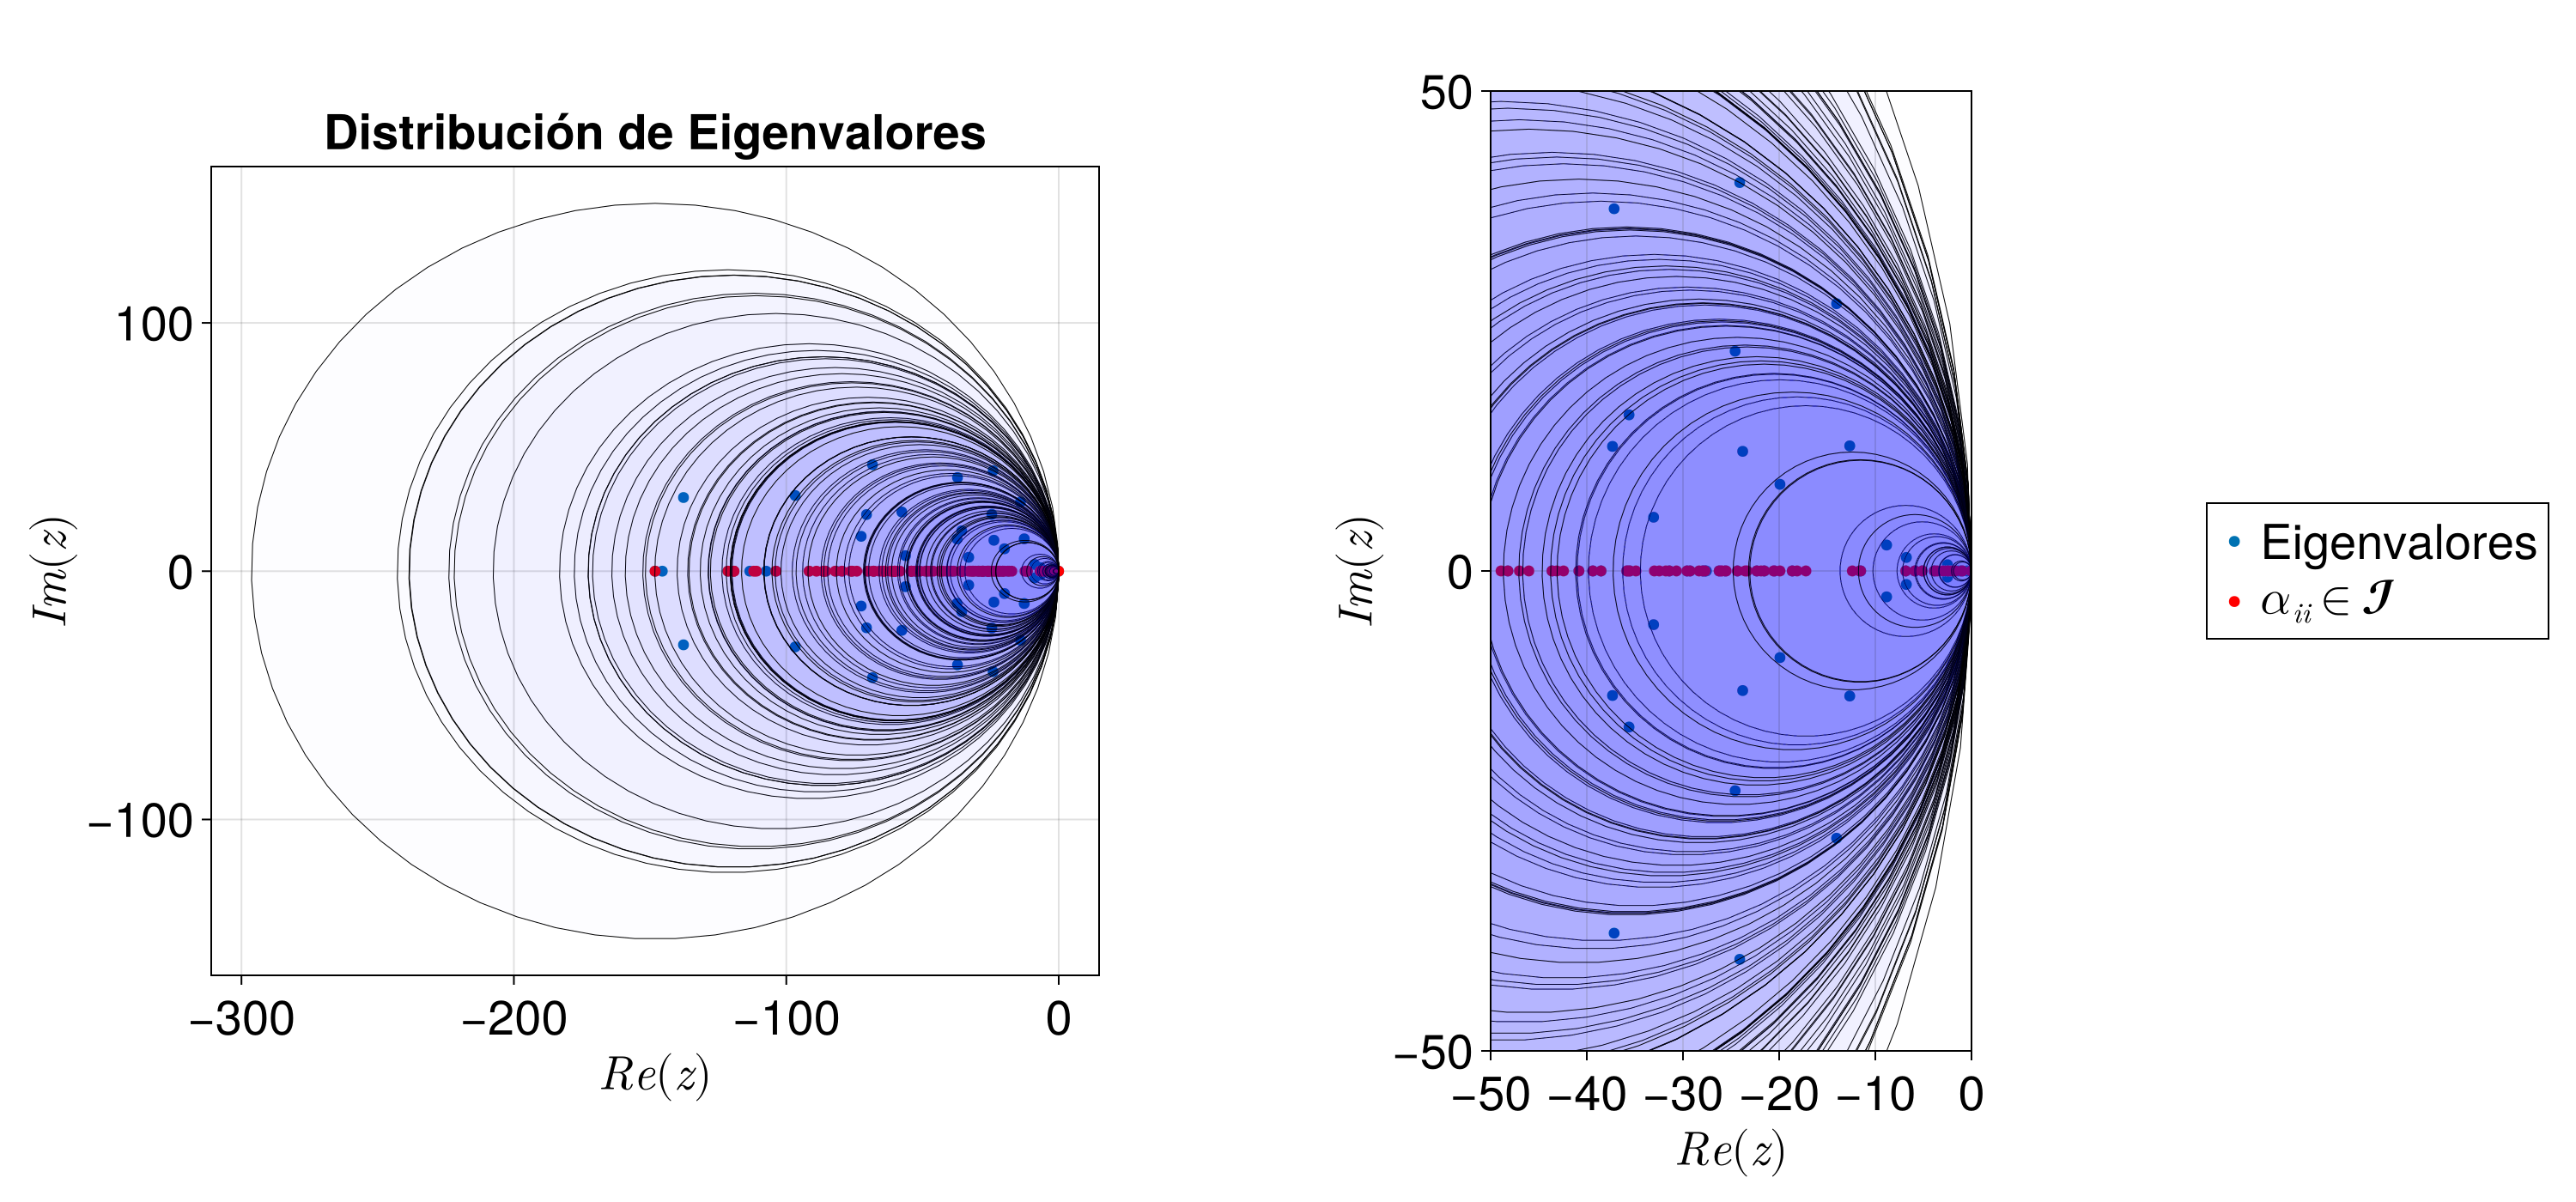
\includegraphics[scale=0.17]{../Imagenes/LeyesCirculares}
	\caption{Distribución de valores propios del sistema generalizado para $N=100$, $\sigma=0.2$ y $p=0.6$. Se consideran $N$ Leyes Circulares cuyo centro y radio es cada valor de la diagonal de la matriz Jacobiana asociada. }
	\label{fig:LeyesCirculares}
\end{figure}


\begin{wrapfigure}{l}{0.5 \textwidth} \vspace{-40pt} \begin{center}
	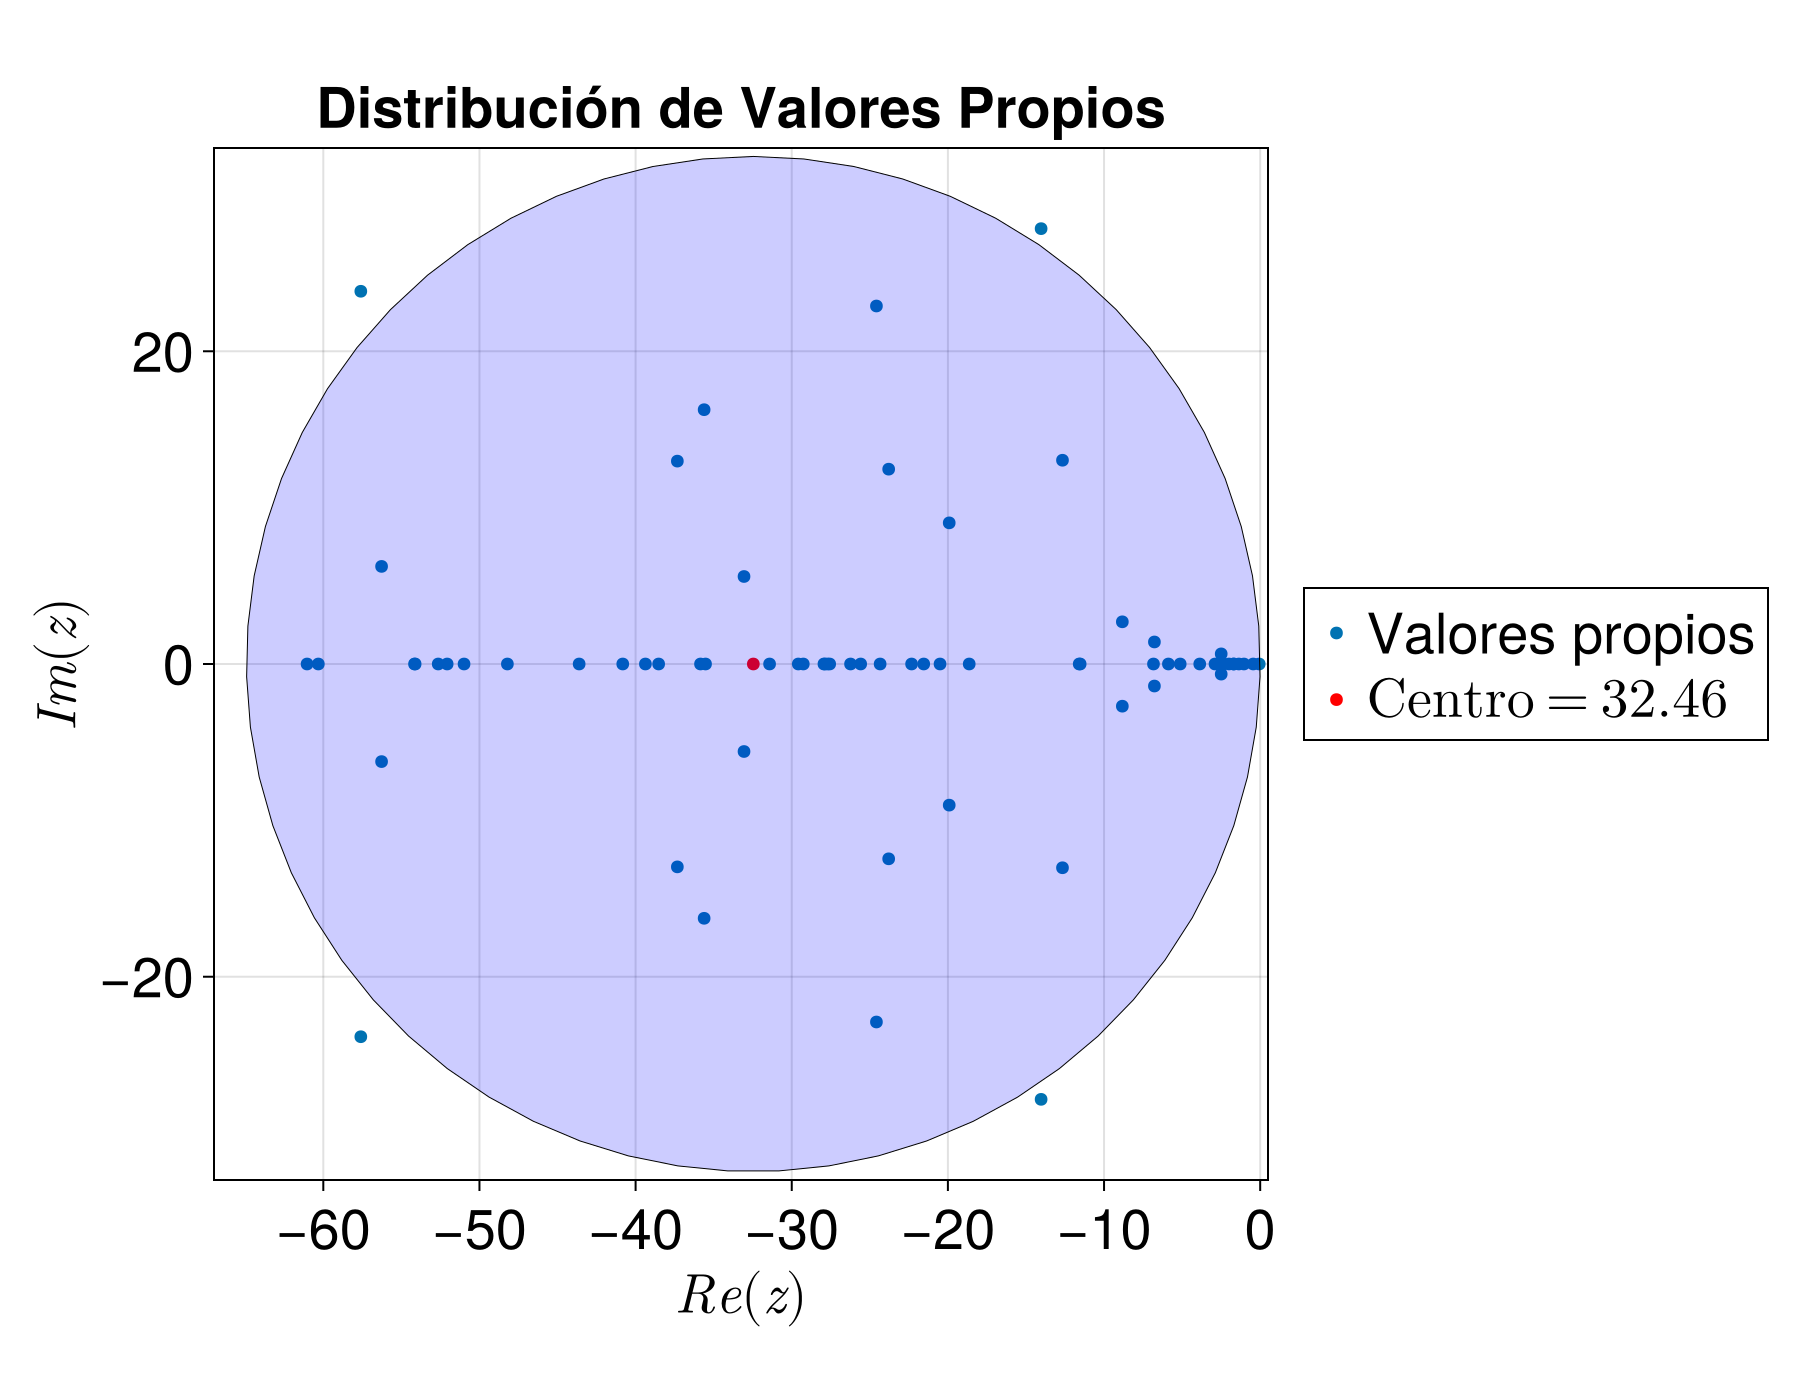
\includegraphics[scale=0.13]{../Imagenes/LeyCircularParticular}
	\end{center}
	\vspace{-20pt} 
	\caption{Caso particular de la Figura (\ref{fig:LeyesCirculares}) para el valor de la diagonal $\alpha_{ii}=32.46\in\mathcal{J}$.}
		\vspace{-10pt}
	\label{fig:LeyCircularParticular}
\end{wrapfigure}
Esta propuesta se inspira de la Proposición \ref{prop:DiagonalI}, en donde se invocaron los discos de Gershgorin que se encuentran centrados en cada valor de la diagonal de $\mathcal{J}$ y se demuestra que los radios pueden ser menores o iguales a cada uno de estos valores. Al ser menores o iguales, la actual propuesta toma el máximo caso posible (es decir la igualdad) y por lo tanto cada círculo encerrará un porcentaje de valores propios que se encuentren en la vecindad alrededor de $\mathcal{J}_{ii}$ de mismo radio.\\
\\
Un caso particular de la Figura (\ref{fig:LeyesCirculares}) considerando $\mathcal{J}_{ii}=32.46$ se puede observar en la Figura (\ref{fig:LeyCircularParticular}), cierto porcentaje de valores propios se distribuye por el círculo varios concentrados en el eje real solamente, sin embargo existen algunos otros que se escapan del confinamiento particular y pasan al siguiente nivel o círculo. Para poder confirmar o refutar esta propuesta, se explorarán múltiples sistemas estables con sus respectivas distribuciones de diagonales y valores propios.

\subsection{Análisis para $N=50$}

Se tienen a disposición dos conjuntos de datos, ambos son de simulaciones realizadas para diferentes valores de $p$ y $\sigma$. Cada conjunto esta conformado por 78 archivos .csv y son simulaciones de matrices \href{https://github.com/rogve98/Tesis/tree/master/Notebooks/Datos/Jacobianos}{Jacobianas} y de distribuciones de \href{https://github.com/rogve98/Tesis/tree/master/Notebooks/Datos/Diagonales}{Diagonales}\footnote{Para los Jacobianos acceder a: \url{https://github.com/rogve98/Tesis/tree/master/Notebooks/Datos/Jacobianos}. Para las Diagonales acceder a \url{https://github.com/rogve98/Tesis/tree/master/Notebooks/Datos/Diagonales}.}. Así mismo, en cada archivo se encuentran 100 simulaciones que resultaron estables y de los cuales se realizará el análisis correspondiente a la relación entre la distribución de las diagonales y de las partes reales de los valores propios de las matrices Jacobianas. En la siguiente tabla se muestra el esquema de simulaciones para cada $p$ y $\sigma$
\begin{table}[h!]
	\centering
	\begin{tabular}{|c|c|c|c|}
		\hline
		Fuerza promedio [$\sigma$] & Probabilidades [$p$] & Cantidad de archivos & Simulaciones realizadas \\ \hline
		$0.1-0.5$  & $0.1-1.0$  & 50 & 5000  \\ \hline
		0.6  & $0.1-0.9$  & 9 & 900 \\ \hline
		0.7  & $0.1-0.7$  & 7 & 700 \\ \hline
		0.8  & $0.1-0.5$  & 5 & 500 \\ \hline
		0.9  & $0.1-0.4$  & 4 & 400 \\ \hline
		1.0  & $0.1-0.3$  & 3 & 300 \\ \hline
		& \textbf{Total:} & 78& 7800\\ \hline
	\end{tabular}
	\caption{Cantidad de archivos generados para el banco de Diagonales y Jacobianos considerando $N=50$. A partir de $\sigma=0.6$ en adelante, los tiempos de compilación fueron muy prolongados por lo que no se obtuvieron los 10 archivos respectivos a diferencia de los valores promedio anteriores.}
	\label{tab:Simulaciones}
\end{table} 

La razón principal de escoger los sistemas para $N=50$ es por el costo computacional. Ha resultado muy prolongado el tiempo de compilación de sistemas más grandes (como el de $N=100$) y aún así para valores altos de la fuerza promedio ($\sigma\geq 0.6$) no se obtuvieron los 10 archivos por la misma razón. Habiendo introducido la información experimental, se procede a continuar con el análisis de las $N$ Leyes Circulares. Para ello convendrá determinar la correlación entre estas cantidades así como apreciar una comparativa visual entre la parte real y los valores de la diagonal.
\newpage
\begin{figure}[h!]
	\centering
	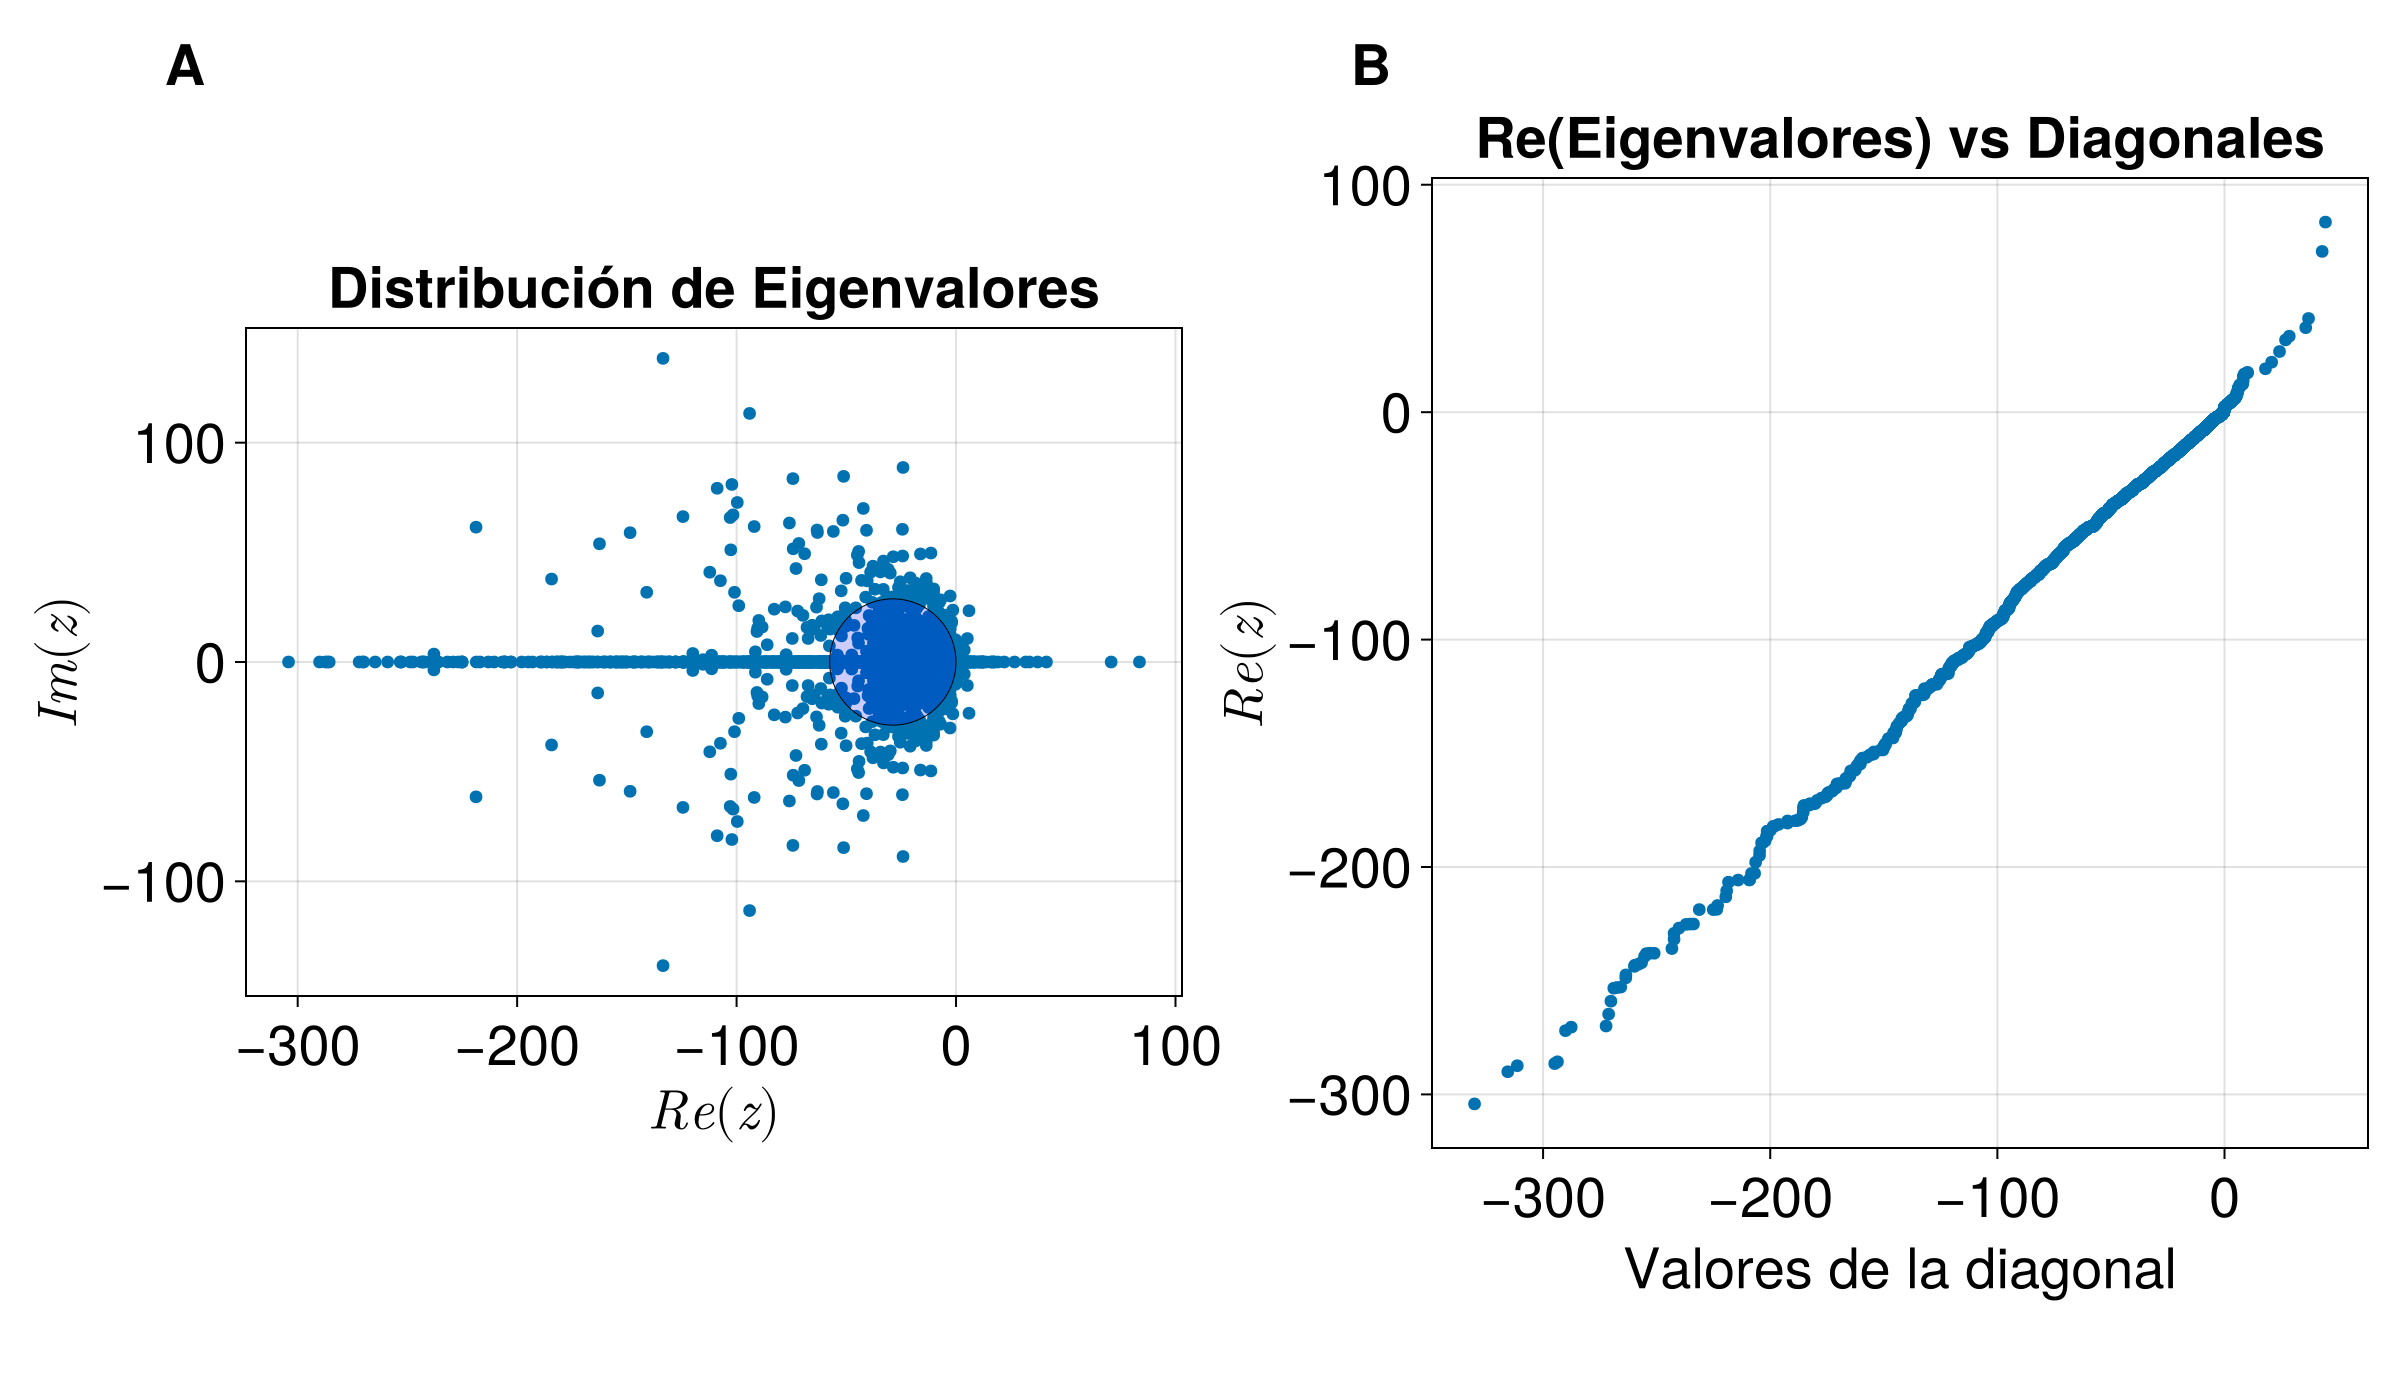
\includegraphics[scale=0.2]{../Imagenes/ReEvs-Diagonales}
	\caption{(\textbf{A}) Distribución de valores propios de 100 jacobianos para el caso $\sigma=0.5$, $p=0.5$. Se agrega una ley circular correspondiente al valor medio de la distribución de diagonales. (\textbf{B}) Relación entre la parte real de los valores propios con las diagonales de los Jacobianos considerados.}
	\label{fig:ReEvs-Diagonales}
\end{figure}

A simple vista se puede observar una relación lineal, y puede ser casi perfecta en algunos casos pero será cuestión de coincidencia, pues los valores propios se encuentran en las vecindades de Gershgorin alrededor de cada entrada de la diagonal de $\mathcal{J}$. Lo que nos muestra la Figura (\ref{fig:ReEvs-Diagonales} \textbf{B}) es que los $|\mathcal{J}_{ii}|$ más grandes de la distribución tienen un rango amplio en el radio de Gershgorin para alojar valores propios, lo que implica que posiblemente la parte real de de estos no se encuentre cerca de dicho valor $\mathcal{J}_{ii}$ y que por lo tanto no exista una relación tan lineal en estos casos.  A diferencia de los $|\mathcal{J}_{ii}|$ de menor tamaño que parecen tener un radio de Gershgorin proporcional y que ello implique que los valores propios se alojen cerca de dicho centro $\mathcal{J}_{ii}$ pudiendo marcar una mejor relación lineal. Más adelante se mostrará un ejemplo más evidente de este hecho.\\
\\
En la Figura (\ref{fig:ReEvs-Diagonales} \textbf{A}) se ha agregado una Ley Circular particular con centro y radio correspondiente al valor medio de la distribución, esto con el fin de observar que tan significativa es la media de la distribución en cuanto a ver cuantos valores propios es capaz de encerrar. Aunque encierra una gran cantidad de ellos, también un gran porcentaje queda fuera por lo que la media no es un valor representativo de la distribución en este caso. Para seguir explorando si la relación lineal existe también para el resto de las simulaciones de la Tabla (\ref{tab:Simulaciones}) se tomará la media, mediana y moda de las distribuciones de diagonales $d(\sigma_i,p_j)$ y partes reales de los conjuntos de valores propios $\overline{\lambda}$ para compararlos viendo si existe una correspondencia lineal entre estas cantidades.
\begin{figure}[h!]
	\centering
	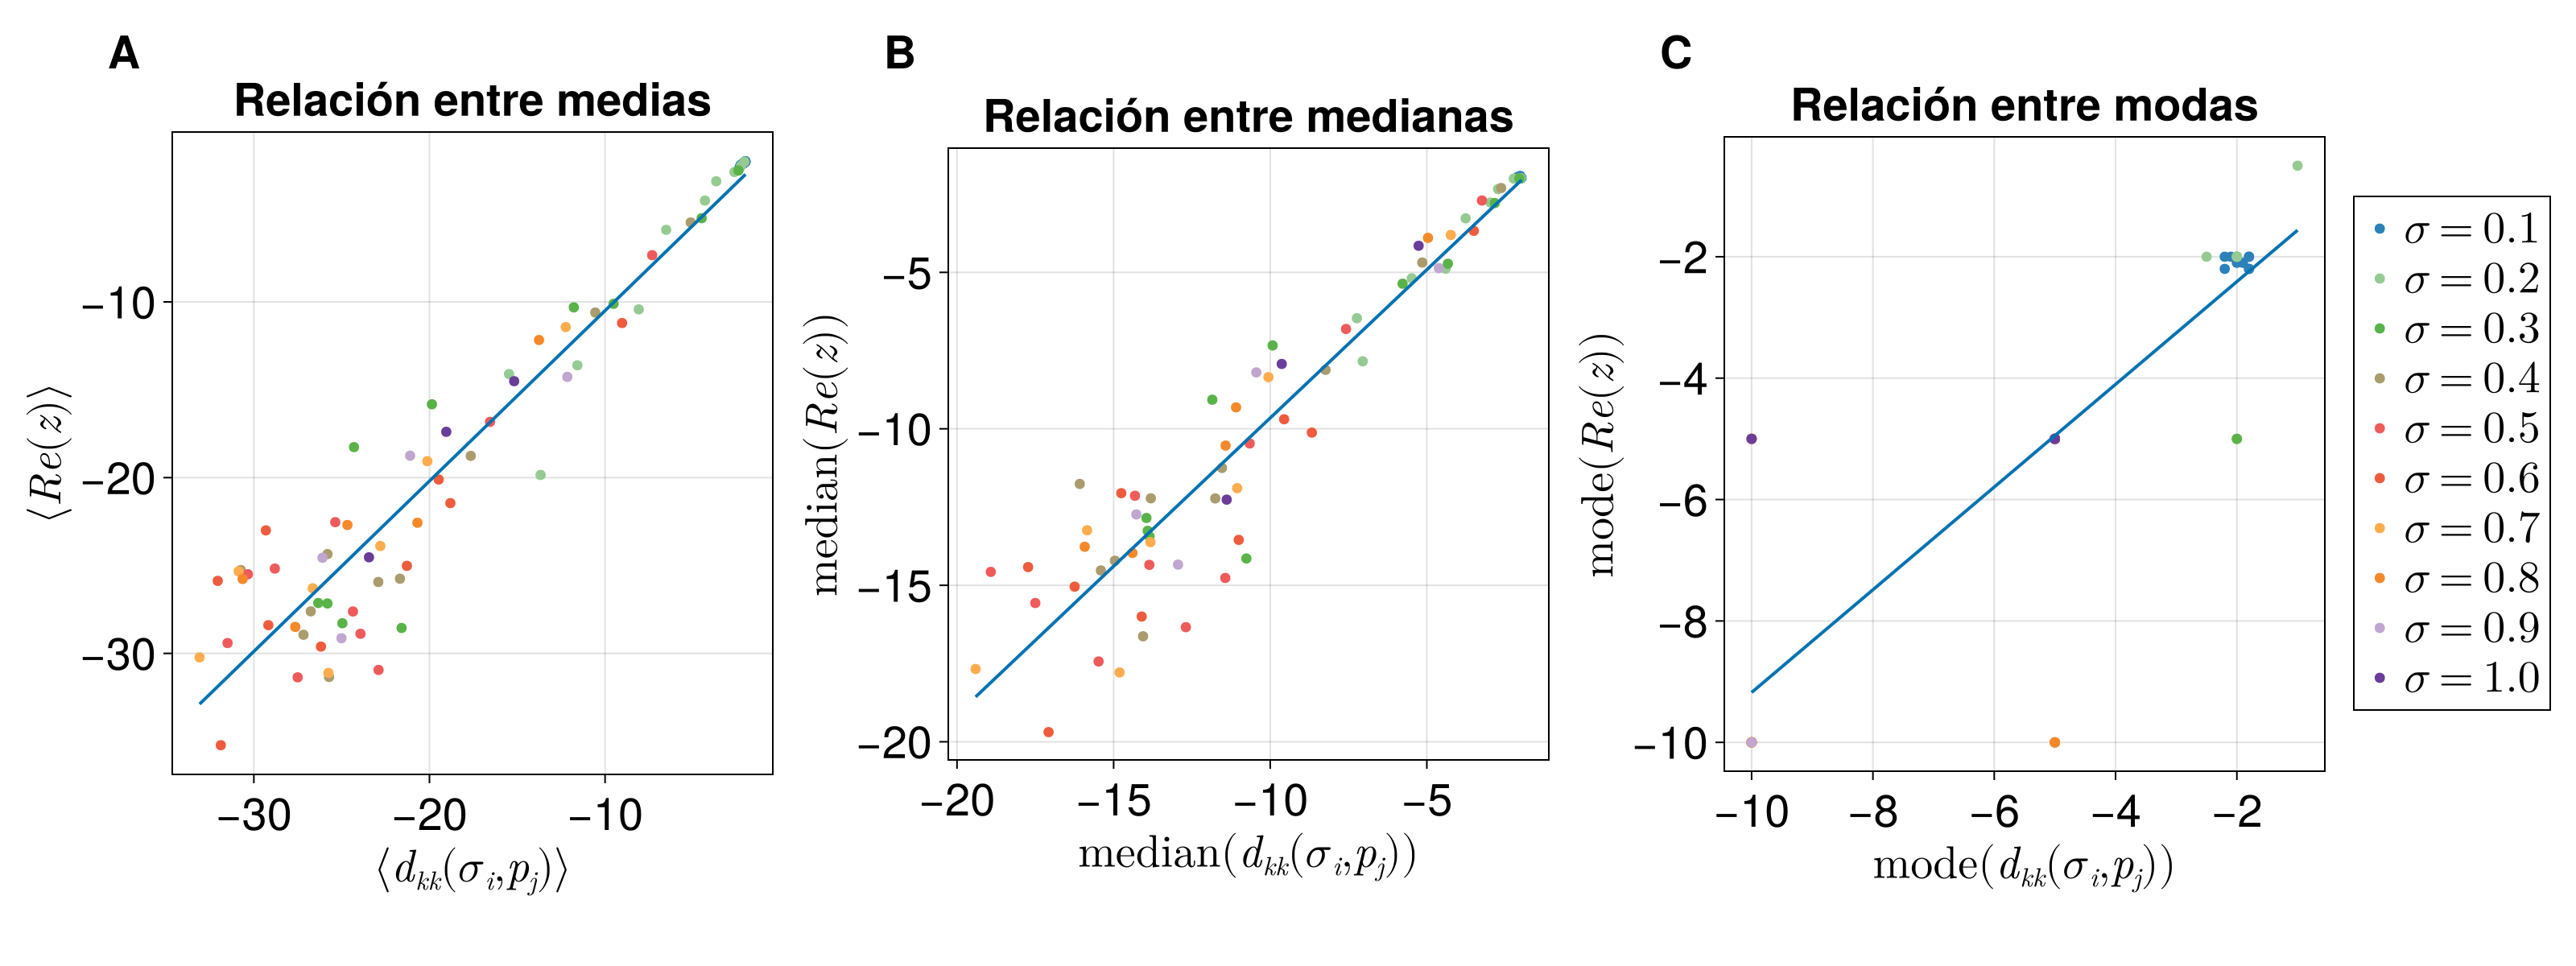
\includegraphics[scale=0.16]{../Imagenes/AjustesLinMeds}
	\caption{(\textbf{A}) Ajuste lineal de la relación entre las medias de las $Re(\overline{\lambda})$ con las medias de las $\mathcal{J}_{kk}(\sigma_i,p_j)$ de los Jacobianos del sistema. (\textbf{B}) Ajuste lineal de la relación entre las medianas $Re(\overline{\lambda})$ con las medianas de las $d_{kk}(\sigma_i,p_j))$ de los Jacobianos del sistema. (\textbf{C}) Ajuste lineal de la relación entre las modas de $Re(\overline{\lambda})$ con las modas de las $d_{kk}(\sigma_i,p_j)$ de los Jacobianos del sistema.}
	\label{fig:AjustesLinMeds}
\end{figure}
\newpage
\section{Transiciones de estabilidad}

Para darle seguimiento a los resultados de esta tesis, ésta sección se va a centrar en explorar cuales son las condiciones de la matriz de incidencias (en función de $\sigma$, $p$ y $N$) para que los Jacobianos resultantes muestren estabilidad o no. Recordando una de las conclusiones de May: un sistema será estable si la conectancia del sistema (dada por $p$) es débil mientras que la fuerza de las interacciones (dada por $\sigma$) es considerablemente alta; y ésto es válido en sentido opuesto, si dicha fuerza es baja entonces existe la oportunidad de que el sistema sea estable con una alta conectividad. \\
\\
Para ello se van a considerar tres tipos de sistemas, para $N=\{100,50,25\}$. Se pretende ver que tanto cambia la estabilidad con diferentes tamaños del sistema (\ref{eqn:LK}). La metodología que se va a aplicar para resolver este problema es la siguiente: Para cada $N$ se va a realizar exactamente lo mismo salvo algunas variaciones, primero se va a integrar el sistema fijando la fuerza de interacción en los siguientes valores $\tilde{\sigma}=\{0.1,0.2,...,1.0\}$ mientras que para las probabilidades de conectividad se va a considerar la siguiente partición del intervalo $[0,1]$ para cada $N$:
\begin{equation}\label{eqn:particionLin}
	p = \{x_i\, |\, x_i=i\cdot\Delta x, i=0,1,2,...,100\},\qquad\text{con }\Delta x=0.01
\end{equation}
Con esta configuración de valores se permitirá generar diagramas de transición de estabilidad para cada $N$ en función de $p$ considerando que es una partición equidistante. Hay otros dos diagramas de estabilidad que son de interés; siguiendo en función de la probabilidad de conectividad se define la siguiente partición sobre el intervalo $[0,1]$
\begin{equation}\label{eqn:particionLog}
	p_{\log}=\left \{ x_i\, |\, x_i=10^{-\left (10-\frac{10i}{99}\right )},\ i=0,1,...,99\right \}
\end{equation}
Se ha considerado particularmente este conjunto de probabilidades de conectividad ya que para ciertas $\sigma$ y para $N=100$ primordialmente, la transición ocurre de manera abrupta de tal modo que en la escala lineal no se aprecia cuando ocurre la transición, por ende se permite visualizar este cambio para valores muy pequeños. Más adelante se irá viendo este fenómeno. Por último pero no menos importante, se van a considerar diagramas en donde se deja fija la $p$ para cada $N$ y se define una partición equidistante en el intervalo $[0,1]$ en función de la fuerza de interacción, es decir:
\begin{equation}
	\sigma = \{x_i\, |\, x_i=i\cdot\Delta x, i=0,1,2,...,100\},\qquad\text{con }\Delta x=0.01
\end{equation}
Para esta configuración de valores se obtendrán los diagramas de transición en función de $\sigma$ y se verá que tan contrastante es con respecto de los otros diagramas de transición. Teniendo las particiones y los ajustes de parámetros necesarios para generar los diagramas de transición, solamente falta ver cómo y de qué manera se van a generar estos diagramas. Para cada $N$, $\sigma$ y $p$ con sus correspondientes particiones se va a integrar el sistema cierto número de veces por cada elemento de ésta misma:
\newpage
\begin{table}[h!]
	\centering
	\begin{tabular}{|c|c|}
		\hline
		Tamaño del sistema $N$ & Cantidad de simulaciones por cada elemento de la partición  \\ \hline
		100 & 3000 \\ \hline
		50  & 6000 \\ \hline
		25  & 12000 \\ \hline		
 	\end{tabular}
	\caption{Cantidad de simulaciones realizadas por cada $N$ y para cada elemento de la partición definida.}
	\label{tab:SimulacionesTransicion}
\end{table} 

De tal forma que se van a determinar cuantos sistemas resultaron estables del total de simulaciones realizadas para dicho elemento y se van a contabilizar. Al final de cuentas esto nos brinda un porcentaje de estabilidad el cual se irá visualizando en sus respectivos diagramas de transición, y lo que se estará observando es que a medida que los valores de la partición aumentan, la estabilidad de los sistemas es cada vez menor. La elección de cada cantidad de simulaciones por elemento de partición, responde a la intención de suavizar las curvas, entre más valores se consideren la curva se hace cada vez más suave; con pocos puntos las curvas no se visualizan suaves. De esta forma, entre más chico sea el tamaño del sistema se requieren mas simulaciones para poder suavizar dicha curva.\\
\\
En una primera versión de resultados se consideró un método que generó algunos problemas los cuales se visualizaron en la sección anterior, en la discusión de los sistemas asintótica-mente estables: los cuales no alcanzaron su estabilidad o quizás no eran estables y todo gracias al tiempo de integración de $t_f=50$. Sin embargo se han generado otros resultados en donde se pone una restricción para que solamente se consideren sistemas que se integren en un tiempo máximo de $t_f=50$. Entre ambos tipos de resultados existen algunas desviaciones que requerirán de su análisis más adelante.\\
\\
Habiendo conseguido los diagramas de transición mediante todo un proceso computacionalmente arduo, merece preguntarse si acaso estas transiciones corresponden con transiciones de fase, y de ser cierto ¿cuál sería su parámetro crítico? Se tiene una pista en la relación (\ref{eqn:parametroMay}) que re acomodando se tiene
\begin{equation}\label{eqn:ParametroCritico}
	\sigma\sqrt{NC}<d
\end{equation}
donde en el caso de May corresponde con la diagonal fijada en $-d=-1$. Se explorará si en los diagramas de transición generados existe alguna dependencia/relación con algún valor representativo de las $d_{kk}(\sigma_i,p_j)$ de los Jacobianos del sistema.

\section{Para $N=100$}

holaaaa